\appendix
\section{Appendix}

\subsection*{Pseudocode}
\label{app:pseudocode}
%E-step
\begin{algorithm}[H]
    \caption{E-step: Computation of Responsibilities}
    \begin{algorithmic}[1]
        \Require Dataset $X \in \mathbb{R}^{N \times D}$, parameters $\mu_{k}, \sigma_{k}, \pi_{k}$ for $k=1,\dots,K$
        \Ensure Responsibilities $\gamma_{ik}$
        \For{$i = 1$ to $N$}
            \State $\text{denom} \gets 0$
            \For{$k = 1$ to $K$}
                \State $\gamma_{ik}  \gets \pi_k \cdot \mathcal{N}(X[i] \mid \mu_k, \Sigma_k)$ \Comment{Gaussian density using \ref{gaussian_alg}}
                \State $\text{denom} \gets \text{denom} + \gamma_{ik}$
            \EndFor

            \For{$k = 1$ to $K$}
                \State $\gamma_{ik} \gets \gamma_{ik} / \text{denom}$ 
        \EndFor
        \EndFor
    \end{algorithmic}
    \label{e_step_alg}
\end{algorithm}

%M-step
\begin{algorithm}[H]
    \caption{M-step: Parameter Update}
    \begin{algorithmic}[1]
        \Require Dataset $X \in \mathbb{R}^{N \times D}$, responsibilities $\gamma_{ik}$
        \Ensure Updated parameters $\mu_k$, $\sigma_k$, $\pi_k$
        \State Initialize accumulators: $N_k \gets 0$, $\mu^{\text{acc}}_{kd} \gets 0$, $\sigma^{\text{acc}}_{kd} \gets 0$
        \For{$i = 1$ to $N$}
            \For{$k = 1$ to $K$}
                \State $N_k \gets N_k + \gamma_{ik}$
                \For{$d = 1$ to $D$}
                    \State $\mu^{\text{acc}}_{kd} \gets \mu^{\text{acc}}_{kd} + \gamma_{ik} \cdot X[i,d]$
                \EndFor
            \EndFor
        \EndFor
        \For{$k = 1$ to $K$}
            \For{$d = 1$ to $D$}
                \State $\mu_{kd} \gets \mu^{\text{acc}}_{kd} / N_k$
            \EndFor
        \EndFor
        \For{$i = 1$ to $N$}
            \For{$k = 1$ to $K$}
                \For{$d = 1$ to $D$}
                    \State $\sigma^{\text{acc}}_{kd} \gets \sigma^{\text{acc}}_{kd} + \gamma_{ik} \cdot (X[i,d] - \mu_{kd})^2$
                \EndFor
            \EndFor
        \EndFor
        \For{$k = 1$ to $K$}
            \For{$d = 1$ to $D$}
                \State $\sigma_{kd} \gets \sigma^{\text{acc}}_{kd} / N_k$
            \EndFor
            \State $\pi_k \gets N_k / N$
        \EndFor
    \end{algorithmic}
    \label{m_step_alg}
\end{algorithm}

%Multivariate Gaussian Density with Diagonal Covariance
\begin{algorithm}[H]
    \caption{Compute multivariate Gaussian density with diagonal covariance}
    \begin{algorithmic}[1]
        \Require $x \in \mathbb{R}^D$, $\mu \in \mathbb{R}^D$, $\sigma \in \mathbb{R}^D$ 
        \Ensure $\mathcal{N}(x \mid \mu, \sigma)$
        \State $\text{logdet} \gets 0$
        \State $\text{quad} \gets 0$
        \For{$d = 1$ to $D$}
            \State $var \gets \sigma[d]$
            \State $\text{logdet} \gets \text{logdet} + \log(var)$
            \State $\text{diff} \gets x[d] - \mu[d]$
            \State $\text{quad} \gets \text{quad} + \frac{\text{diff}^2}{var}$
        \EndFor
        \State $\text{exponent} \gets -0.5 \cdot ( D \cdot \log 2\pi + \text{logdet} + \text{quad} )$
        \State \Return $\exp(\text{exponent})$
    \end{algorithmic}
    \label{gaussian_alg}
    \caption{Gaussian Density Computation with Diagonal Covariance}
\end{algorithm}

%Clustering Label Assignment
\begin{algorithm}[H]
    \caption{Clustering: Label Assignment from Responsibilities}
    \begin{algorithmic}[1]
        \Require Responsibilities matrix $\gamma \in \mathbb{R}^{N \times K}$
        \Ensure Predicted labels $\hat{y} \in \{1,\dots,K\}^N$
        \For{$i = 1$ to $N$}
            \State $\text{max\_resp} \gets \gamma_{i1}$ \Comment{Initialize with first cluster responsibility}
            \State $\hat{y}_i \gets 1$
            \For{$k = 2$ to $K$}
                \If{$\gamma_{ik} > \text{max\_resp}$}
                    \State $\text{max\_resp} \gets \gamma_{ik}$
                    \State $\hat{y}_i \gets k$
                \EndIf
            \EndFor
        \EndFor
    \end{algorithmic}
\label{clustering_alg}
\end{algorithm}

\subsection*{Other Datasets Full Results}

\begin{figure}[H]
    \centering
    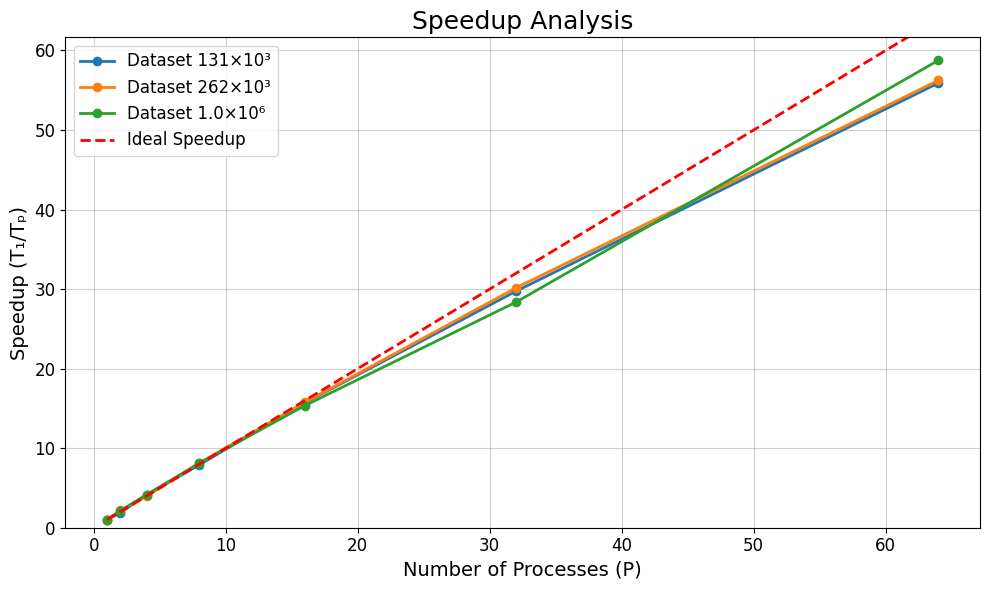
\includegraphics[width=1\textwidth]{../media/mpi_speedup_other.png}
    \caption{Speedup plot for different dataset sizes (small, medium, large) with increased features and clusters. The dashed line represents the ideal linear speedup.}
    \label{fig:mpi_speedup_plot_other}
\end{figure}

\subsection*{Hybrid Full Results}
Here are the complete results for the Hybrid approach, including execution time, speedup, and E-Step efficiency.
\begin{table}[H]
    \centering
    \renewcommand{\arraystretch}{1.2}
    \setlength{\tabcolsep}{4pt}
    \footnotesize
    \begin{tabularx}{\textwidth}{c|*{7}{>{\centering\arraybackslash}X}}
        \hline
        \textbf{N\_Processes} & \textbf{0.033M} & \textbf{0.066M} & \textbf{0.131M} & \textbf{0.262M} & \textbf{0.524M} & \textbf{1.049M} &\textbf{2.097M} \\
        \hline
        1  & 633.233 & 1177.423 & 2191.697 & 4637.819 & 8652.474 & 17008.507 & 30070.722 \\
        2  & 304.441 & 603.905 & 1113.554 & 2354.183 & 4471.163 & 8265.101 & 17905.912 \\
        4  & 147.311 & 278.408 & 565.111 & 1085.605 & 2265.491 & 4041.279 & 8094.882 \\
        8  & 75.020 & 149.955 & 280.005 & 579.793 & 1085.627 & 2048.421 & 4145.526 \\
        16 & 39.447 & 79.223 & 155.722 & 324.658 & 590.897 & 1151.906 & 2186.361 \\
        32 & 20.313 & 42.183 & 82.698 & 149.456 & 304.556 & 588.653 & 1143.465 \\
        64 & 10.694 & 21.348 & 40.104 & 78.604 & 148.252 & 296.361 & 541.036 \\
        \hline
    \end{tabularx}
    \caption{Execution Time (seconds) for different dataset sizes and number of processes.}
\label{tab:execution_time_hybrid}
\end{table}

\begin{table}[H]
    \centering
    \renewcommand{\arraystretch}{1.2}
    \setlength{\tabcolsep}{4pt}
    \footnotesize
    \begin{tabularx}{\textwidth}{c|*{7}{>{\centering\arraybackslash}X}}
        \hline \textbf{N\_Processes} &  \textbf{0.033M} &  \textbf{0.066M} &  \textbf{0.131M} &  \textbf{0.262M} &  \textbf{0.524M} &  \textbf{1.049M} & \textbf{2.097M} \\
        \hline
        1  & 1.000 & 1.000 & 1.000 & 1.000 & 1.000 & 1.000 & 1.000 \\
        2  & 2.080 & 1.950 & 1.968 & 1.970 & 1.935 & 2.058 & 1.679 \\
        4  & 4.299 & 4.229 & 3.878 & 4.272 & 3.819 & 4.209 & 3.715 \\
        8  & 8.441 & 7.852 & 7.827 & 7.999 & 7.970 & 8.303 & 7.254 \\
        16 & 16.053 & 14.862 & 14.074 & 14.285 & 14.643 & 14.766 & 13.754 \\
        32 & 31.173 & 27.912 & 26.503 & 31.031 & 28.410 & 28.894 & 26.298 \\
        64 & 59.214 & 55.155 & 54.650 & 59.002 & 58.363 & 57.391 & 55.580 \\
        \hline
    \end{tabularx}
    \caption{Speedup (T1/Tp) for different dataset sizes and number of processes.}
\label{tab:speedup_hybrid}
\end{table}

\begin{figure}[H]
    \centering
    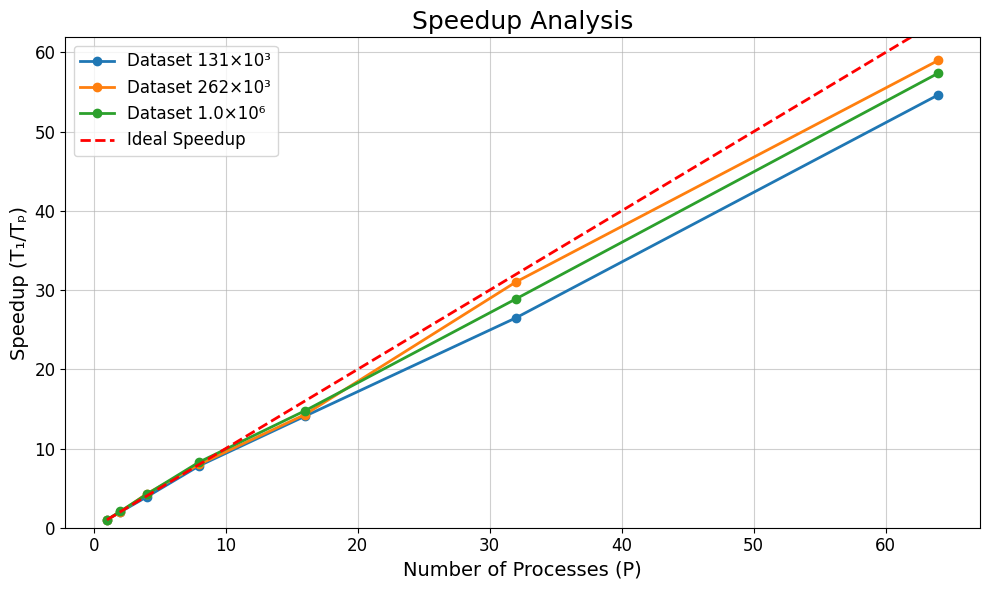
\includegraphics[width=1\textwidth]{../media/hybrid_speedup.png}
    \caption{Hybrid Speedup plot for different dataset sizes (small, medium, large). The dashed line indicates the ideal linear speedup.}
    \label{fig:hybrid_speedup_plot_2}
\end{figure}

\begin{table}[H]
    \centering
    \renewcommand{\arraystretch}{1.2}
    \setlength{\tabcolsep}{4pt}
    \footnotesize
    \begin{tabularx}{\textwidth}{c|*{7}{>{\centering\arraybackslash}X}}
        \hline \textbf{N\_Processes} &  \textbf{0.033M} &  \textbf{0.066M} &  \textbf{0.131M} &  \textbf{0.262M} &  \textbf{0.524M} &  \textbf{1.049M} & \textbf{2.097M} \\
        \hline
        1  & 1.000 & 1.000 & 1.000 & 1.000 & 1.000 & 1.000 & 1.000 \\
        2  & 1.040 & 0.977 & 0.984 & 0.982 & 0.966 & 1.024 & 0.845 \\
        4  & 1.074 & 1.058 & 0.970 & 1.067 & 0.957 & 1.050 & 0.935 \\
        8  & 1.055 & 0.982 & 0.979 & 1.001 & 0.994 & 1.036 & 0.917 \\
        16 & 1.013 & 0.935 & 0.898 & 0.929 & 0.919 & 0.937 & 0.872 \\
        32 & 0.984 & 0.896 & 0.854 & 0.990 & 0.902 & 0.913 & 0.845 \\
        64 & 0.948 & 0.895 & 0.863 & 0.955 & 0.924 & 0.914 & 0.893 \\
        \hline
    \end{tabularx}
    \caption{E-Step efficiency for different dataset sizes and number of processes.}
\label{tab:efficiency_estep_hybrid}
\end{table}